% GNUPLOT: LaTeX picture with Postscript
\begingroup
  \makeatletter
  \providecommand\color[2][]{%
    \GenericError{(gnuplot) \space\space\space\@spaces}{%
      Package color not loaded in conjunction with
      terminal option `colourtext'%
    }{See the gnuplot documentation for explanation.%
    }{Either use 'blacktext' in gnuplot or load the package
      color.sty in LaTeX.}%
    \renewcommand\color[2][]{}%
  }%
  \providecommand\includegraphics[2][]{%
    \GenericError{(gnuplot) \space\space\space\@spaces}{%
      Package graphicx or graphics not loaded%
    }{See the gnuplot documentation for explanation.%
    }{The gnuplot epslatex terminal needs graphicx.sty or graphics.sty.}%
    \renewcommand\includegraphics[2][]{}%
  }%
  \providecommand\rotatebox[2]{#2}%
  \@ifundefined{ifGPcolor}{%
    \newif\ifGPcolor
    \GPcolortrue
  }{}%
  \@ifundefined{ifGPblacktext}{%
    \newif\ifGPblacktext
    \GPblacktexttrue
  }{}%
  % define a \g@addto@macro without @ in the name:
  \let\gplgaddtomacro\g@addto@macro
  % define empty templates for all commands taking text:
  \gdef\gplbacktext{}%
  \gdef\gplfronttext{}%
  \makeatother
  \ifGPblacktext
    % no textcolor at all
    \def\colorrgb#1{}%
    \def\colorgray#1{}%
  \else
    % gray or color?
    \ifGPcolor
      \def\colorrgb#1{\color[rgb]{#1}}%
      \def\colorgray#1{\color[gray]{#1}}%
      \expandafter\def\csname LTw\endcsname{\color{white}}%
      \expandafter\def\csname LTb\endcsname{\color{black}}%
      \expandafter\def\csname LTa\endcsname{\color{black}}%
      \expandafter\def\csname LT0\endcsname{\color[rgb]{1,0,0}}%
      \expandafter\def\csname LT1\endcsname{\color[rgb]{0,1,0}}%
      \expandafter\def\csname LT2\endcsname{\color[rgb]{0,0,1}}%
      \expandafter\def\csname LT3\endcsname{\color[rgb]{1,0,1}}%
      \expandafter\def\csname LT4\endcsname{\color[rgb]{0,1,1}}%
      \expandafter\def\csname LT5\endcsname{\color[rgb]{1,1,0}}%
      \expandafter\def\csname LT6\endcsname{\color[rgb]{0,0,0}}%
      \expandafter\def\csname LT7\endcsname{\color[rgb]{1,0.3,0}}%
      \expandafter\def\csname LT8\endcsname{\color[rgb]{0.5,0.5,0.5}}%
    \else
      % gray
      \def\colorrgb#1{\color{black}}%
      \def\colorgray#1{\color[gray]{#1}}%
      \expandafter\def\csname LTw\endcsname{\color{white}}%
      \expandafter\def\csname LTb\endcsname{\color{black}}%
      \expandafter\def\csname LTa\endcsname{\color{black}}%
      \expandafter\def\csname LT0\endcsname{\color{black}}%
      \expandafter\def\csname LT1\endcsname{\color{black}}%
      \expandafter\def\csname LT2\endcsname{\color{black}}%
      \expandafter\def\csname LT3\endcsname{\color{black}}%
      \expandafter\def\csname LT4\endcsname{\color{black}}%
      \expandafter\def\csname LT5\endcsname{\color{black}}%
      \expandafter\def\csname LT6\endcsname{\color{black}}%
      \expandafter\def\csname LT7\endcsname{\color{black}}%
      \expandafter\def\csname LT8\endcsname{\color{black}}%
    \fi
  \fi
  \setlength{\unitlength}{0.0500bp}%
  \begin{picture}(7200.00,5040.00)%
    \gplgaddtomacro\gplbacktext{%
      \csname LTb\endcsname%
      \put(1430,2904){\makebox(0,0)[r]{\strut{} 1}}%
      \csname LTb\endcsname%
      \put(1430,3273){\makebox(0,0)[r]{\strut{} 10}}%
      \csname LTb\endcsname%
      \put(1430,3642){\makebox(0,0)[r]{\strut{} 100}}%
      \csname LTb\endcsname%
      \put(1430,4010){\makebox(0,0)[r]{\strut{} 1000}}%
      \csname LTb\endcsname%
      \put(1430,4379){\makebox(0,0)[r]{\strut{} 10000}}%
      \csname LTb\endcsname%
      \put(1562,2684){\makebox(0,0){\strut{} 0}}%
      \csname LTb\endcsname%
      \put(2086,2684){\makebox(0,0){\strut{} 1000}}%
      \csname LTb\endcsname%
      \put(2610,2684){\makebox(0,0){\strut{} 2000}}%
      \csname LTb\endcsname%
      \put(3134,2684){\makebox(0,0){\strut{} 3000}}%
      \csname LTb\endcsname%
      \put(3658,2684){\makebox(0,0){\strut{} 4000}}%
      \csname LTb\endcsname%
      \put(4183,2684){\makebox(0,0){\strut{} 5000}}%
      \csname LTb\endcsname%
      \put(4707,2684){\makebox(0,0){\strut{} 6000}}%
      \csname LTb\endcsname%
      \put(5231,2684){\makebox(0,0){\strut{} 7000}}%
      \csname LTb\endcsname%
      \put(5755,2684){\makebox(0,0){\strut{} 8000}}%
      \csname LTb\endcsname%
      \put(6279,2684){\makebox(0,0){\strut{} 9000}}%
      \csname LTb\endcsname%
      \put(6803,2684){\makebox(0,0){\strut{} 10000}}%
      \put(176,3641){\rotatebox{-270}{\makebox(0,0){\strut{}Frontera}}}%
      \put(396,3641){\rotatebox{-270}{\makebox(0,0){\strut{}(Escala Logaritmica)}}}%
      \put(4182,2354){\makebox(0,0){\strut{}Cantidad de Nodos}}%
      \put(4182,2134){\makebox(0,0){\strut{}(Escala Lineal)}}%
      \put(4182,4709){\makebox(0,0){\strut{}Relacion Frontera/Nodos}}%
    }%
    \gplgaddtomacro\gplfronttext{%
      \csname LTb\endcsname%
      \put(6263,1713){\makebox(0,0)[r]{\strut{}Primer Vecino}}%
      \csname LTb\endcsname%
      \put(6263,1493){\makebox(0,0)[r]{\strut{}Primer Vecino con golosa}}%
      \csname LTb\endcsname%
      \put(6263,1273){\makebox(0,0)[r]{\strut{}Primer Vecino con intercambio}}%
      \csname LTb\endcsname%
      \put(6263,1053){\makebox(0,0)[r]{\strut{}Primer Vecino con intercambio y golosa}}%
      \csname LTb\endcsname%
      \put(6263,833){\makebox(0,0)[r]{\strut{}Mejor Vecino}}%
      \csname LTb\endcsname%
      \put(6263,613){\makebox(0,0)[r]{\strut{}Mejor Vecino con golosa}}%
      \csname LTb\endcsname%
      \put(6263,393){\makebox(0,0)[r]{\strut{}Mejor Vecino con intercambio}}%
      \csname LTb\endcsname%
      \put(6263,173){\makebox(0,0)[r]{\strut{}Mejor Vecino con intercambio y golosa}}%
    }%
    \gplbacktext
    \put(0,0){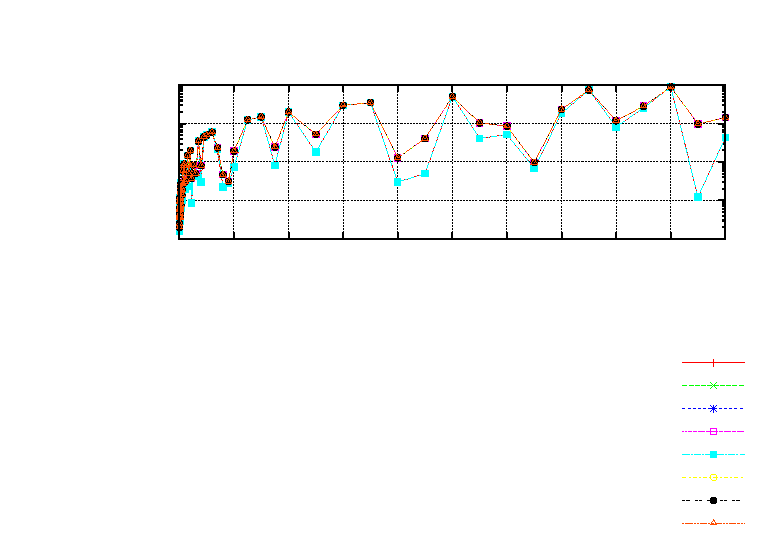
\includegraphics{ej3_frontera_banana}}%
    \gplfronttext
  \end{picture}%
\endgroup
